\documentclass[english, 11pt]{article}

\usepackage{notes}
\usepackage{epigraph}

% Uncomment these for a different family of fonts
% \usepackage{cmbright}
% \renewcommand{\sfdefault}{cmss}
% \renewcommand{\familydefault}{\sfdefault}

%\newcommand{\thiscoursecode}{[XXXX] (\#\#\#)}
\newcommand{\thiscoursename}{Quantum Mechanics}
\newcommand{\thisprof}{Ivan Iorsh}
\newcommand{\me}{Pavel Dmitriev}
\newcommand{\thisterm}{Autumn 2015}
%\newcommand{\website}{MYWEBSITE.COM}

% Headers
\chead{\thiscoursename \ Course Notes}
\lhead{\thisterm}


%%%%%% TITLE %%%%%%
\newcommand{\notefront} {
	\pagenumbering{roman}
	\begin{center}
	
		%{\ttfamily \url{\website}} {\small}
		
		%\textbf{\Huge{\noun{\thiscoursecode}}}{\Huge \par}
		
		{\Huge{\noun{\thiscoursename}}}\\ \vspace{0.1in}
		
		{\noun \thisprof} \ $\bullet$ \ {\noun \thisterm} \ $\bullet$ \ {\noun {ITMO University}} \\
	
	\end{center}
}

% Begin Document
\begin{document}

	% Notes front
	\notefront
	% Table of Contents and List of Figures
	\tocandfigures
	% Abstract
	\doabstract{Quantum Mechanics Lecture Notes.}
	
	\section{Introduction}
	\subsection{Schr\"odinger formalism}
	
		\begin{equation}
			\hat{f}\Phi =  E \Phi
		\end{equation}
	
		\begin{equation}
			\Phi \rightarrow dP = |\Phi|^2dq
		\end{equation}
		
		\begin{equation}
			x \leftrightarrow \hat{x}
		\end{equation}

		\begin{equation}
			p_x \leftrightarrow -i\hbar \frac{\partial}{\partial x}
		\end{equation}
	
		\begin{equation}
			f \leftrightarrow \hat{f}
		\end{equation}	
		
		\begin{equation}
			\bar{f} = \int \hat{f}dp = \int \Phi^* \hat{f} \Phi dq 
		\end{equation}
	
	\subsection{Heisenberg formalism}
		\epigraph{Schr\"odinger was good at math, which is why his quantum mechanics formalism is full of complex mathematical constructs. Heisenberg, on the other hand, had a lot of difficulty with math, which is why his matrix quantum mechanics formalism is limited almost exclusively to linear algebra constructs}{Roman ... }
	
		\begin{tabular}{c | c | c }
			Name & Schr\"odinger & Heisenberg \\
			\hline
			\hline
			\ &&\\
			
			 State Basis & Wave function of basis states $ \{ \Phi_n \} $ & Column vector of basis states $\begin{pmatrix}\phi_1\\...\\ \phi_n\end{pmatrix}$ \\[3ex]		
			\hline
			\hline
			\ &&\\
			
			Observables & Operator $ \bar{f} = \int \Phi_n^* \hat{f} \Phi_m$ & Operator matrix $\begin{pmatrix}\phi_{11} & ... & \phi_{n1} \\ & ... & \\ \phi_{1n} & ... & \phi_{nn}\end{pmatrix}$ \\[3ex]
			\hline
			\hline
			
			\ &&\\
			Shr\"odinger Equation & $ \hat{f}\Phi =  E \Phi$ & $\begin{pmatrix}\phi_{11} & ... & \phi_{n1} \\ & ... & \\ \phi_{1n} & ... & \phi_{nn}\end{pmatrix} \begin{pmatrix}\psi_1\\...\\ \psi_n\end{pmatrix} = \lambda \begin{pmatrix}\psi_1\\...\\ \psi_n\end{pmatrix}$ \\[3ex]
			\hline
			\hline			
		\end{tabular}
	
		\subsubsection{Building an operator's matrix}
			For a system with a discrete state basis, $\{\Psi_n \}$, any state of the system can be described as a linear combination of the basis' wave functions:
			
			\begin{equation}
				\Psi = \sum_{n}a_n\Psi_n
			\end{equation}
			
			Observable $\bar{f}$  for such a wave function can be decomposed into a sum over the basis state wave functions:
			
			\begin{align}
				\bar{f} = & \int \Psi^* \hat{f} \Psi dq = \int \sum_{n}a_n^*\Psi_n^* \hat{f} \sum_{m}a_m\Psi_m dq \nonumber \\ 
				=  &\sum_{n}\sum_{m}a_n^* a_m \int \Psi_n^* \hat{f} \Psi_m dq = \sum_{n}\sum_{m}a_n^* a_m f_{nm}(t) \nonumber \\
				=  &\sum_{n}\sum_{m}a_n^* f_{nm}(t) a_m
			\end{align}
			
			Where $f_{nm}$ is the operator matrix.
			
			\subsubsection{$f_nm(t)$ time dependence}
				\hl{Move to appendix?}
				
				Solutions to the time-independent Shr\"odinger equation: 
				\begin{align}
					\hat{H}\Psi_n &= E_n \Psi_n \\
					\Psi_n(t) &= e^{-\frac{i}{\hbar}E_n t} \Phi_n
				\end{align}
				
				Which, in operator matrix terms translates into

				\begin{align}
					f_{nm}(t) &= \int \Psi_n^* \hat{f} \Psi_m dq = \int \Phi_n^* (e^{-\frac{i}{\hbar}E_n t})^* \hat{f} \Phi_m e^{-\frac{i}{\hbar}E_m t} dq \nonumber\\
					&=  e^{+\frac{i}{\hbar}E_n t}e^{-\frac{i}{\hbar}E_m t} \int \Phi_n^*\hat{f} \Phi_m  dq = e^{i \frac{E_n-E_m}{\hbar} t} \int \Phi_n^*\hat{f} \Phi_m  dq \nonumber\\
					&= f_{nm} e^{i \omega_{nm} t} 		
				\end{align}
				
			\subsubsection{Operator matrix properties}
				\begin{enumerate}
					\item The operator matrix is hermitian \footnote{$H^\dag = H = (H^*)^T$}
						Transposed operator:
						\begin{equation}
							(\int \Phi \hat{f} \Psi dq \quad)^T = \int \Psi (\hat{f})^T \Phi dq
						\end{equation}
						Complex conjugate:
						\begin{equation}
							(\hat{f})^* = \hat{f^*}
						\end{equation}	
						Hermitian conjugate:
						\begin{equation}
							\bar{f^*} = \int \Psi^* \hat{f}^\dag \Psi dq
						\end{equation}
						
						In operator matrix terms:
						\begin{align}
							(f_{nm}^*) &= \int \varphi_n^* \hat{f}^\dag \varphi_m dq = \int \varphi_n^* (\hat{f}^*)^T \varphi_m dq \nonumber \\
							&= \int \varphi_m (\hat{f}^* \varphi_n^*) dq = (\int \varphi_m^* \hat{f}^\dag \varphi_n dq )^* = (f_{mn})^*
						\end{align}
						Which means, if $f_{nm}$ is real, meaning $f_{nm}^* = f_{nm}$ that
						\begin{equation}
							f_{nm} = f_{mn}^* = f_{nm}^\dag
						\end{equation}
					\item The matrix' diagonal elements are time-independent and real
						\begin{equation}
							f_{nn} = \int \Psi_n \hat{f} \Psi_n dq \equiv \bar{f}_{n}
						\end{equation}
						
						Where $\bar{f}_{n}$ is the value of observable $f$ in basis state $n$.
						
					\item The matrix of the product of two operators is the product of their matrices
					
						For operators $\hat{f}$ and $\hat{g}$, what is the operator matrix for operator $\hat{f}\times\hat{g}$ ~--- $(\hat{f}\times\hat{g})_{nm}$?

						\hl{Move to appendix?}						
						\begin{align}
							\hat{f}\varphi_n &= \sum_m f_{mn} \varphi_m \\
							\int \varphi_k^* dq \times \hat{f}\varphi_n &=  \int \varphi_k^* dq \times \sum_m f_{mn} \varphi_m \nonumber \\
							\int \varphi_k^* \hat{f}\varphi_n dq &= \sum_m f_{mn} \int \varphi_k^* \varphi_m dq
							f_{kn} = \sum_m f_{mn} \delta_{km} = f_{kn}
						\end{align}
						Because for state basis ${\varphi_n}$, $\varphi_n$ and $\varphi_m$ are orthogonal for all $m \not= n$.
						
						Using 1.18, we can write:
						\begin{align}
							\hat{f}\hat{g}\varphi_n &= \hat{f}(\hat{g}\varphi_n) = \hat{f} \sum_k g_kn \varphi_k = \sum_k g_{kn} \hat{f} \varphi_k \nonumber \\
							&= \sum_k g_{kn} \sum_m f_{mk} \varphi_m = \sum_{k,m} g_{kn}f_{mk}\varphi_m \nonumber \\ 
							&= \sum_{k,m} f_{mk}g_{kn}\varphi_m
						\end{align}
						And knowing that:
						\begin{equation}
							(\hat{f}\hat{g})\varphi_n = \sum_m(\hat{f}\hat{g})_{nm}\varphi_m
						\end{equation}
						We end up with:
						\begin{equation}
							(\hat{f}\hat{g})_{mn} = \sum_k f_{mk}g_{kn}
						\end{equation}
						
					\item The operator's matrix is equivalent to the operator
				\end{enumerate}
	
			\subsection{Switching to a different state basis}
		
	
	\subsection{Pauli uncertainty principle}
		\subsubsection{Single-slit electron diffraction}
		\subsubsection{Black holes}
		\subsubsection{Quantum Pencil}
			\cite{easton2007quantum}
		
	\subsection{Problems}
	\section{Analytical Solutions}
	\subsection{Rectangular quantum well}
	\subsection{Harmonic oscillator}
	\subsection{Spherically symmetric potential}

	\section{Quasi-classical approximation}
	\subsection{Problems}
  
	\section{Spin}
	\subsection{Angular momentum}
		\subsubsection{Classical}
			\begin{figure}[!h]
				\centering
				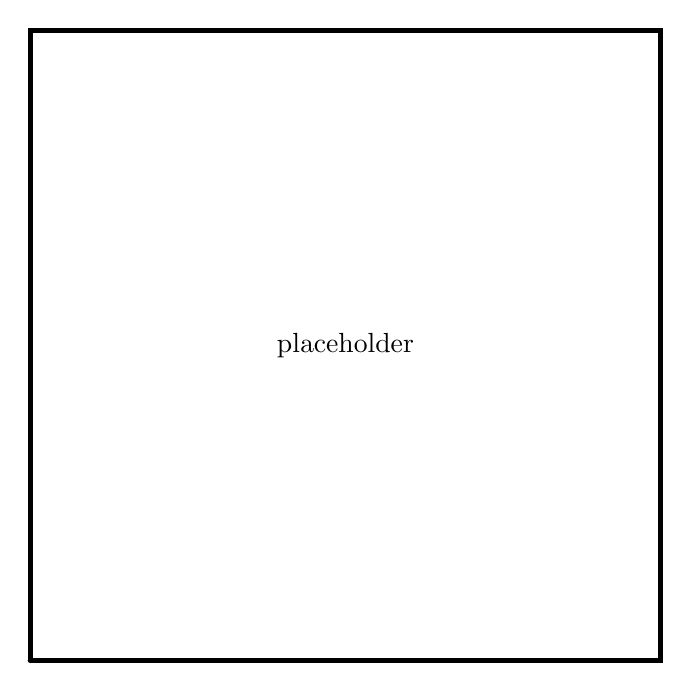
\begin{tikzpicture}[scale=2,cap=round,>=latex]
	\draw [line width=2] (-2, -2) -- (-2, 2) -- (2, 2) -- (2, -2) -- (-2, -2);
	
	\node at (0, 0) {placeholder};
\end{tikzpicture}
				\caption{Classical angular momentum}
				\label{clasmoment}
			\end{figure}
			
			\begin{align}
				\vec{L} =& \vec{r}\times\vec{p} =
				\begin{vmatrix}
					\vec{e_x} & \vec{e_y} & \vec{e_z} \\
					x & y & z \\
					p_x & p_y & p_z \\
				\end{vmatrix} \\
				=& \vec{e_x}(yp_z - zp_y) + \vec{e_y}(zp_x - xp_z) + \vec{e_z}(xp_y - yp_x) \\
				=& \vec{e_x}L_x + \vec{e_y}L_y + \vec{e_z}L_z
			\end{align}
			
			%Building on classical angular momentum is the Rutherford atomic model:
			%\begin{figure}[!h]
			%	\centering
			%	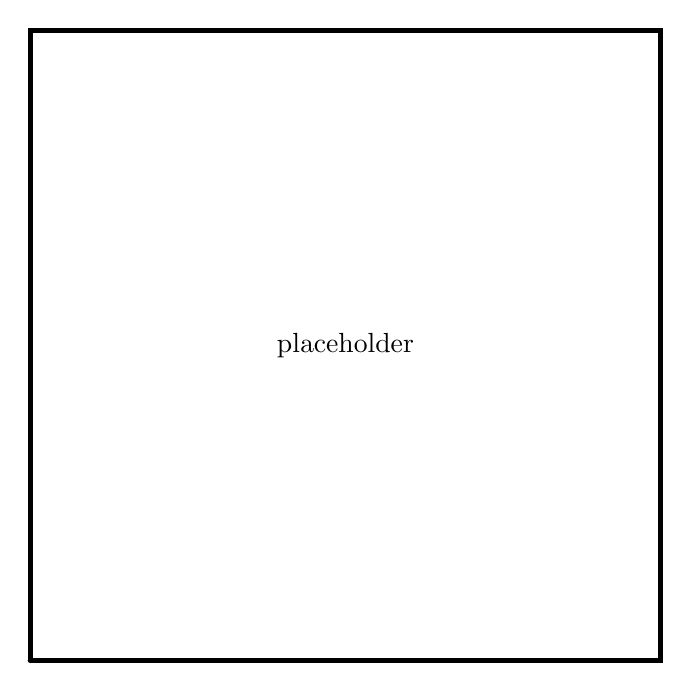
\begin{tikzpicture}[scale=2,cap=round,>=latex]
	\draw [line width=2] (-2, -2) -- (-2, 2) -- (2, 2) -- (2, -2) -- (-2, -2);
	
	\node at (0, 0) {placeholder};
\end{tikzpicture}
			%	\caption{Rutherford atom}
			%	\label{ruthatom}
			%\end{figure}
			%
			%\begin{align}
			%	\frac{mv^2}{r} =& \frac{ke^2}{r^2} \\
			%	m\vec{a} =& \vec{F_c}
			%\end{align}
			%
			%\begin{list}[Problems with the Rutherford model]
			%	\item Discrete energy levels
			%	\item 
			%\end{list}
		\subsubsection{Quantum}
			\begin{align}
				\hat{\vec{p}} =& -i\hbar\vec{\nabla}, \qquad \vec{\nabla} = \vec{e_x}\frac{\partial}{\partial x} + \vec{e_y}\frac{\partial}{\partial y} + \vec{e_z}\frac{\partial}{\partial z} \\
				p_x =& -i\hbar \frac{\partial}{\partial x}, \quad p_y = -i\hbar \frac{\partial}{\partial y}, \quad p_z = -i\hbar \frac{\partial}{\partial z} \\
				\hat{\vec{L}} =& -i\hbar\vec{r}\times\vec{\nabla} \\
				\hat{L_x} =& -i\hbar(y\frac{\partial}{\partial z} - z\frac{\partial}{\partial y}), \quad \hat{L_y} = -i\hbar(z\frac{\partial}{\partial x} - x\frac{\partial}{\partial z}), \quad \hat{L_z} = -i\hbar(y\frac{\partial}{\partial x} - x\frac{\partial}{\partial y}) 
			\end{align}
			
			\hl{Proof!} Commutators:
			\begin{equation}
				\left[\hat{L_x}, \hat{L_y}\right] = i\hbar\hat{L_z}, \quad
				\left[\hat{L_z}, \hat{L_x}\right] = i\hbar\hat{L_y}, \quad
				\left[\hat{L_y}, \hat{L_z}\right] = i\hbar\hat{L_x}
			\end{equation}
			
			Uncertainty: \hl{Wait, what?}
			\begin{align}
				\Delta \hat{L_x} = \hat{L_x} - \left<\hat{L_x} \right>, \quad
				\Delta \hat{L_y} = \hat{L_y} - \left<\hat{L_y} \right>, \quad
				\Delta \hat{L_z} = \hat{L_z} - \left<\hat{L_z} \right> \\
				\left<(\Delta\hat{L_x})^2 \right> = \left<\hat{L_x}^2 \right> - \left<\hat{L_x} \right>^2 \\
				\left<(\Delta\hat{L_y})^2 \right> = \left<\hat{L_y}^2 \right> - \left<\hat{L_y} \right>^2 \\
				\left<\hat{L_x} \right> = \int \Psi^* \hat{L_x} \Psi dV \\ 
				\left<(\Delta\hat{L_x})^2 \right>\left<(\Delta\hat{L_y})^2 \right> \geq \frac{\hbar^2|\left<\hat{L_z}\right>|^2}{4} \\
				\left<(\Delta x)^2 \right>\left<(\Delta p_x)^2 \right> \geq \frac{\hbar^2}{4} \nonumber				
			\end{align}
			
			Generally it isn't possible to measure $L_x, L_y, L_z$ at once. 
		
	\subsection{Problems}    
	\section{Perturbation theory}    
	\subsection{Time-independent}
	\subsection{Time-dependent}
	\section{Problem Solutions}
	\subsection{Introduction}
	\subsection{Analytical solutions}
	\subsection{Quasiclassical approximation}
	\subsection{Spin}			
	\subsection{Petrubation theory}				
	
	\newpage
	\phantomsection
	\addcontentsline{toc}{section}{References}
	\bibliographystyle{ieeetr}
	\bibliography{references}
	%%%%%%%%%%%%%%%%%%%%%%%%%%%%%%%%%%%%%%%%%%%%%%%
\end{document}
